% !TeX TS-program = lualatex
% !BIB TS-program = biber

\documentclass[a4paper,12pt,openany]{book}
\usepackage[margin=3cm]{geometry}
\usepackage{microtype}
\usepackage{graphicx}
\usepackage{subcaption}
\usepackage{parskip}
\usepackage[table,xcdraw]{xcolor}
\usepackage{array}
\usepackage{tikz}
\usepackage[labelfont=bf]{caption}
\usepackage{float}
\newcommand{\imagesource}[1]{{\footnotesize Source: #1}}
% "toc" posa "Appendices" a l'índex.
% "page" posa la pàgina "Appendices" abans del primer annex.
\usepackage[]{appendix}
% pseudocode
\usepackage[ruled,algochapter]{algorithm2e}
\SetKwBlock{QuotientCode}{code $q$}{end}
\SetKwBlock{RemainderCode}{code $r$}{end}

% Acronyms
\usepackage[toc,acronym]{glossaries}
\makeglossaries

\usepackage[hidelinks]{hyperref}

% Change text font
\usepackage{fontspec}
\usepackage{amssymb}
%\usepackage{unicode-math}
%\setmainfont{Libertinus Serif}
%\setmathfont{Libertinus Math}

\newtheorem{theorem}{Theorem}
\numberwithin{theorem}{chapter}
\DeclareMathOperator{\EX}{\mathbb{E}}

% Use biblatex to manage bibliography.
\usepackage[
	backend=biber,
	style=alphabetic,
	sorting=nyt,
	urldate=iso,
	date=iso
]{biblatex}
\addbibresource{bibliography.bib}
% Increase space between bibliography items.
\setlength\bibitemsep{0.3\baselineskip}

% Set custom headers and footers.
\usepackage{fancyhdr}
\fancypagestyle{plain} {
	\fancyhf{}
	\renewcommand{\headrulewidth}{0pt}
	\renewcommand{\footrulewidth}{1pt}
	\fancyfoot[RO, LE]{\thepage}
}
\pagestyle{fancy}
\fancyhf{}
\renewcommand{\headrulewidth}{1.5pt}
\renewcommand{\footrulewidth}{1pt}
\fancyhead[LE]{\leftmark}
\fancyhead[RO]{\rightmark}
\fancyfoot[RO, LE]{\thepage}

% Change space before, between and after chapter title.
\usepackage{titlesec}
\titleformat{\chapter}[display]
{\normalfont\huge\bfseries}{\chaptertitlename\ \thechapter}{0pt}{\Huge}
\titlespacing*{\chapter}{0pt}{-20pt}{15pt}

% Enable or disable my comments
\usepackage{ifthen}
\usepackage{comment}
\specialcomment{comment}{\begingroup \color{blue}}{\endgroup}
\newboolean{showcomment}
\setboolean{showcomment}{true} % Comment to disable block comments
\ifthenelse{\boolean{showcomment}}{}{\excludecomment{comment}}


\begin{document}
\newacronym{fapec}{FAPEC}{Fully Adaptive Prediction Error Coder}
\newacronym{rf}{RF}{Radio Frequency}
\newacronym{gnss}{GNSS}{Global Navigation Satellite System}
\newacronym{ro}{RO}{Radio Occultation}
\newacronym{flac}{FLAC}{Free Lossless Audio Codec}
\newacronym{iq}{IQ}{In-phase \& Quadrature}
\newacronym{mwc}{MWC}{Multibeam Water Column}
\newacronym{sdr}{SDR}{Software Defined Radio}
\newacronym{wav}{WAV}{Waveform Audio Format}
\newacronym{ccsds}{CCSDS}{Consultative Committee for Space Data Systems}
\newacronym{lsb}{LSB}{Least Significant Bits}
\newacronym{ansi}{ANSI}{American National Standards Institute}
\newacronym{api}{API}{Application Programming Interface}
\newacronym{aes}{AES}{Advanced Encryption Standard}
\newacronym{lzw}{LZW}{Lempel-Ziv-Welch}
\newacronym{dwt}{DWT}{Discrete wavelet transform}
\newacronym{cpu}{CPU}{Central Processing Unit}
\newacronym{wss}{WSS}{Wide-Sense Stationary}
\newacronym{tak}{TAK}{Tom's lossless Audio Kompressor}
\newacronym{upc}{UPC}{Polytechnic University of Catalonia}
\newacronym{ub}{UB}{University of Barcelona}

% Cover.
\frontmatter
\thispagestyle{empty}

\begin{center}
	
\includegraphics[width=\textwidth]{images/logo.png}\\
	
	\vspace*{2.5cm}
	\Huge
	Implementation of FAPEC decorrelation stages for IQ and water column data\\
	
	\vspace*{2.6cm}
	\large
	Degree Thesis\\
	In partial fulfilment of the requirements for the degree in Telecommunications Engineering\\
	
	\vspace*{2cm}
	\textbf{Author}\\
	Aniol Martí Espelt\\
	\vspace*{1.5em}
	\textbf{Advisors}\\
	Ferran de Cabrera Estanyol\\
	Jordi Portell i de Mora\\
	Jaume Riba Sagarra\\
	
	\vspace*{2.5cm}
	Barcelona, June 2021
	
\end{center}

\newpage

% Load abstract, acknowledgments, etc.
\chapter*{Abstract}
 Lorem ipsum dolor sit amet, consectetur adipiscing elit. Pellentesque sed blandit nibh. Suspendisse feugiat vehicula urna, sit amet maximus velit malesuada sit amet. Integer tempus risus maximus neque semper, vitae euismod tortor posuere. Pellentesque rhoncus, augue sit amet porta posuere, tortor turpis auctor lectus, a scelerisque arcu mauris vel leo. Mauris id commodo mi. Ut id magna et dolor ultricies congue. Sed pretium tincidunt rutrum. Vestibulum lacus metus, faucibus eu volutpat eu, cursus sed urna. In laoreet velit a massa varius, at convallis ante efficitur. Fusce eu posuere augue. Vestibulum elementum, tellus ac mattis iaculis, nisi leo posuere enim, eu mollis mi enim eget enim. Proin varius convallis augue, in euismod dui egestas auctor. Curabitur quis varius eros. Donec tortor nulla, fringilla ut pellentesque non, pulvinar non dolor.

Duis ornare commodo nibh eget imperdiet. Donec eu neque eget turpis lacinia gravida. Donec hendrerit, urna convallis dignissim pharetra, odio nibh varius sapien, eu ornare nulla nibh sit amet dolor. Proin commodo ipsum vitae nisi rhoncus, pretium auctor ante euismod. Fusce cursus sapien vel tortor iaculis, a blandit dui volutpat. Sed ut viverra dolor. Duis tempus porta ultrices. Nullam nec purus odio. Interdum et malesuada fames ac ante ipsum primis in faucibus.
\chapter*{Acknowledgments}
\begin{comment}
Lorem ipsum dolor sit amet, consectetur adipiscing elit. Pellentesque sed blandit nibh. Suspendisse feugiat vehicula urna, sit amet maximus velit malesuada sit amet. Integer tempus risus maximus neque semper, vitae euismod tortor posuere. Pellentesque rhoncus, augue sit amet porta posuere, tortor turpis auctor lectus, a scelerisque arcu mauris vel leo. Mauris id commodo mi. Ut id magna et dolor ultricies congue. Sed pretium tincidunt rutrum. Vestibulum lacus metus, faucibus eu volutpat eu, cursus sed urna. In laoreet velit a massa varius, at convallis ante efficitur. Fusce eu posuere augue. Vestibulum elementum, tellus ac mattis iaculis, nisi leo posuere enim, eu mollis mi enim eget enim. Proin varius convallis augue, in euismod dui egestas auctor. Curabitur quis varius eros. Donec tortor nulla, fringilla ut pellentesque non, pulvinar non dolor.

Duis ornare commodo nibh eget imperdiet. Donec eu neque eget turpis lacinia gravida. Donec hendrerit, urna convallis dignissim pharetra, odio nibh varius sapien, eu ornare nulla nibh sit amet dolor. Proin commodo ipsum vitae nisi rhoncus, pretium auctor ante euismod. Fusce cursus sapien vel tortor iaculis, a blandit dui volutpat. Sed ut viverra dolor. Duis tempus porta ultrices. Nullam nec purus odio. Interdum et malesuada fames ac ante ipsum primis in faucibus.
\end{comment}


\tableofcontents
\listoffigures
\listoftables
% Delete blank page between front and mainmatter.
\let\cleardoublepage\clearpage

\mainmatter
\chapter{Introduction}
\section{Objectives}
Lorem ipsum dolor sit amet, consectetur adipiscing elit. Nulla vulputate lectus sit amet quam suscipit convallis. Nulla mattis ipsum eu dapibus commodo. Duis in lacus eget lacus molestie faucibus. Donec aliquet sodales dapibus. Class aptent taciti sociosqu ad litora torquent per conubia nostra, per inceptos himenaeos. Vestibulum ante ipsum primis in faucibus orci luctus et ultrices posuere cubilia curae; Donec metus nulla, consequat at faucibus ac, dignissim vel felis. Suspendisse volutpat sodales justo, quis pulvinar erat laoreet id. Phasellus sed diam sed nunc bibendum ultricies. Aliquam ut ante justo. Nam tincidunt, urna et tristique placerat, quam lectus ultrices arcu, ac laoreet dui massa eget dolor. Aliquam laoreet dolor augue, eu aliquet massa finibus id. Suspendisse vestibulum iaculis sagittis.

Duis tempor dui felis, ac consequat eros pretium eget. Nullam sem lacus, sollicitudin non ipsum eget, ullamcorper vestibulum lectus. Pellentesque euismod metus ac tellus suscipit, a placerat felis consequat. Sed tristique enim eget elit vestibulum ornare nec non libero. Morbi ut elit tincidunt, scelerisque velit maximus, luctus risus. Nulla posuere sem eget tincidunt efficitur. Phasellus neque mi, pulvinar ac vestibulum id, accumsan sed sapien. Ut elementum ac justo a malesuada. Mauris pellentesque sit amet tortor ac hendrerit. Vestibulum ante ipsum primis in faucibus orci luctus et ultrices posuere cubilia curae; Donec accumsan metus a mollis condimentum. Morbi pulvinar mollis consequat. Cras vel velit sed mauris ultrices pellentesque. Pellentesque consequat, eros quis fermentum commodo, ipsum nisl semper est, eleifend congue diam urna vel elit. Mauris rutrum tortor id velit mattis fermentum.

Ut id lacus at risus congue congue. Suspendisse euismod consequat maximus. Suspendisse semper nulla non egestas porttitor. Morbi pulvinar purus tortor, ac placerat enim accumsan vitae. Proin maximus fringilla gravida. Vestibulum luctus lorem arcu, eget dictum enim dictum quis. Maecenas massa urna, sagittis at fringilla quis, dignissim eu mauris. Vivamus a consequat quam. Ut pharetra risus in purus consequat, ut sodales sem aliquet. Sed tortor mi, fermentum eget luctus in, viverra molestie purus. Morbi quis quam eros. Nulla malesuada urna id consectetur pharetra. Suspendisse maximus leo nunc, ut eleifend libero tincidunt ac. Etiam sed sem mauris. Aenean sodales ex nisi, at semper lacus ullamcorper ac.

Nunc at molestie ipsum. Nam efficitur fringilla metus, non finibus mauris tincidunt vel. Curabitur id massa et justo scelerisque ornare nec sed ipsum. Aenean lectus augue, molestie vestibulum ipsum vel, pulvinar facilisis ligula. Vestibulum luctus, libero non porttitor iaculis, magna justo volutpat nisl, vitae tristique sapien nibh in velit. Donec vitae gravida risus, vehicula porttitor eros. Morbi fermentum quis dolor malesuada mollis. Aliquam leo ipsum, vestibulum vel ligula et, pellentesque tincidunt risus. Aliquam dignissim ex ut sollicitudin sagittis. Vivamus augue sem, iaculis porta nunc non, condimentum auctor nisi. Nullam diam tellus, venenatis in rutrum sed, fringilla vel magna. Interdum et malesuada fames ac ante ipsum primis in faucibus. Mauris quis volutpat orci, at feugiat erat. Phasellus vitae nunc ac risus venenatis blandit vitae non nisl. Pellentesque habitant morbi tristique senectus et netus et malesuada fames ac turpis egestas. Donec et tincidunt erat.

Vivamus vel molestie turpis, sit amet efficitur nisl. Donec in porta est, in efficitur neque. Aliquam eu justo commodo, vestibulum mi vel, consequat sem. Morbi sem justo, pellentesque sed massa ut, bibendum facilisis metus. Quisque rhoncus at arcu nec molestie. Suspendisse eget lectus tristique, bibendum diam in, suscipit est. Nunc commodo nunc a purus maximus dignissim. Suspendisse potenti. Maecenas posuere risus nec dui rhoncus tincidunt. Mauris eu ex velit. Cras feugiat, sem ut hendrerit sodales, ligula odio suscipit tellus, bibendum interdum lectus odio semper enim.

Nulla id dignissim velit, a ullamcorper leo. Donec ut tellus vel ipsum molestie suscipit. Curabitur placerat non neque vel facilisis. Morbi in mi iaculis, molestie risus ullamcorper, commodo ex. Sed luctus, arcu at cursus lacinia, felis arcu hendrerit mauris, ac cursus libero justo sed orci. Nulla finibus eleifend libero, a cursus elit congue id. Praesent ultricies elementum eros, vitae aliquam mauris pulvinar ac. Etiam cursus pretium erat, tempor facilisis ipsum elementum id. Nulla blandit nisl ac mi convallis, in maximus justo euismod. Aliquam quis varius purus. Nulla semper sapien sed massa pellentesque fringilla. Pellentesque sagittis id augue at dignissim. Vestibulum ante ipsum primis in faucibus orci luctus et ultrices posuere cubilia curae;

Aliquam consequat, tortor eget mollis fringilla, sapien quam cursus dolor, eu dignissim lacus massa et est. Phasellus elementum magna quam, eu rhoncus velit tincidunt eget. Nunc pretium suscipit ex, vel convallis felis sodales nec. Nunc vitae neque ac felis porttitor varius iaculis vitae augue. Sed finibus lobortis nulla in lacinia. Integer vulputate quis nisl quis semper. Vivamus placerat nisi nunc, eu sollicitudin velit euismod vitae. Proin eu blandit purus. Nunc fermentum vel enim a gravida.

Duis quis lectus non nisl euismod elementum. Vivamus imperdiet consectetur fringilla. Donec vel blandit arcu. Donec luctus aliquam ex vitae aliquet. Fusce tempus ex tristique diam faucibus fringilla. Integer tempus tellus ac mattis euismod. Pellentesque consectetur ipsum nec leo pellentesque tincidunt. Ut leo sapien, dapibus id eleifend at, semper id est. Donec quis sagittis sem. Sed vitae ultricies dolor. Quisque mollis mauris ac malesuada sodales. Nam et laoreet elit. Pellentesque ac justo eros. Phasellus eget velit eu tellus aliquet rhoncus. Aenean laoreet suscipit imperdiet.

Mauris condimentum velit vel nulla semper sollicitudin. Aliquam mi justo, vehicula commodo vulputate in, iaculis vitae neque. Aenean elementum, dolor in hendrerit blandit, ante diam malesuada enim, at convallis nulla lacus vitae sem. Quisque pretium tortor eget aliquam efficitur. Nunc elit erat, interdum nec risus sit amet, consectetur dapibus orci. Praesent vitae congue risus. Nam posuere nisl eget porttitor tincidunt.

Vivamus vitae faucibus urna. Aenean vehicula massa sed nisl dapibus, eu dignissim nulla molestie. Integer non erat dictum, feugiat diam vel, viverra tortor. Pellentesque sit amet iaculis augue. Pellentesque sed enim aliquam, consequat diam in, placerat est. Curabitur porta, eros eget convallis suscipit, metus est tincidunt quam, eget consectetur massa nisl vel lectus. Aliquam pretium, metus id vehicula dignissim, ex massa rutrum ligula, sed dignissim dolor ipsum id erat. Praesent maximus, ex ut consequat elementum, dolor ipsum consectetur ipsum, eu blandit dui mauris non dui.

Morbi in condimentum justo, at facilisis lectus. Donec faucibus neque vitae metus convallis, vitae egestas massa lobortis. Sed non sem sed dolor sollicitudin tempor et blandit massa. In hac habitasse platea dictumst. Morbi sagittis purus nec nisl fringilla, ac lacinia orci iaculis. Phasellus mattis lorem ut blandit luctus. Integer lobortis mauris lacus, nec egestas nulla suscipit in. Phasellus quam nulla, interdum ut rutrum sit amet, malesuada sed eros. Proin et nulla iaculis, fermentum libero at, tempor felis. Aenean in ullamcorper lacus. Donec eu consequat mi. Orci varius natoque penatibus et magnis dis parturient montes, nascetur ridiculus mus. Aliquam erat volutpat. Donec luctus tempor velit, eu dictum erat ornare in. Curabitur vulputate turpis vel dictum placerat. Sed posuere in augue vel posuere.

Suspendisse commodo, magna tincidunt lobortis vestibulum, orci lectus interdum magna, in volutpat velit urna id felis. Fusce eros nibh, hendrerit molestie tincidunt sed, finibus porta velit. Morbi ex velit, sodales eget felis ut, lobortis volutpat arcu. Cras vulputate diam et magna mattis, et cursus eros auctor. Mauris blandit eget ipsum in cursus. In dignissim nunc justo, sed placerat metus ornare ac. Vivamus luctus diam a elit feugiat ultricies. Aenean eu porta dolor, vel molestie arcu. Sed libero diam, lacinia ac vestibulum id, dictum non sapien.

Etiam justo lacus, elementum a odio at, efficitur sagittis urna. Duis nec blandit urna. Cras eleifend porttitor dapibus. Nunc commodo risus vel venenatis accumsan. Etiam quis efficitur diam. Proin suscipit facilisis lorem eget faucibus. Suspendisse felis erat, aliquet sit amet leo sit amet, sodales consequat orci. Nam hendrerit placerat nisi vitae aliquet. Morbi fringilla venenatis nibh sit amet elementum. Donec molestie faucibus maximus. Curabitur in odio imperdiet, placerat nisl vel, cursus purus. Cras sed accumsan enim. Etiam ullamcorper ipsum ac metus posuere, a viverra est porttitor. Nullam venenatis pulvinar orci, quis aliquam mi rutrum at. Duis in leo augue.

Class aptent taciti sociosqu ad litora torquent per conubia nostra, per inceptos himenaeos. Etiam vitae pharetra diam, ac semper risus. Suspendisse sed elit interdum, ullamcorper enim a, vehicula lectus. Nunc a quam pharetra, tristique elit ac, posuere est. Donec finibus pharetra diam non tincidunt. Suspendisse non sem tincidunt, ullamcorper tellus ut, ultricies turpis. Etiam auctor sagittis lacus, sed hendrerit sem. In quis lectus scelerisque, ultrices dolor eget, fringilla est.

Phasellus ac arcu volutpat sem pharetra rutrum. Integer et ante enim. Pellentesque habitant morbi tristique senectus et netus et malesuada fames ac turpis egestas. Vivamus consequat mauris eu mi sollicitudin gravida sit amet ac urna. Praesent fermentum interdum justo, quis lobortis lorem posuere et. Sed suscipit tempus lobortis. Integer maximus nisl eget mauris lacinia, eget imperdiet odio pellentesque. Fusce vitae semper mi. Morbi scelerisque at risus sed tristique. 
\chapter{Entropy Coding}
\begin{comment}
Comentaré alguns algoritmes típics de compressió com el Huffman, Rice-Golomb, codis aritmètics i Asymmetric numeral systems (Zstandard)
\end{comment}

Entropy coding is a lossless data compression scheme based on symbols probability. This field was first described by Claude E. Shannon in 1948 in his paper \textit{A Mathematical Theory of Communication} \parencite{Shannon1948}.

Giving an extensive theoretical explanation of Entropy coding would require an entire thesis, therefore in this chapter we will define the most basic equations in Information Theory and also describe a few well-known coding algorithms that will be relevant later.

\begin{figure}[h!]
	\begin{center}
		\begin{tabular}{ @{} c @{} }
			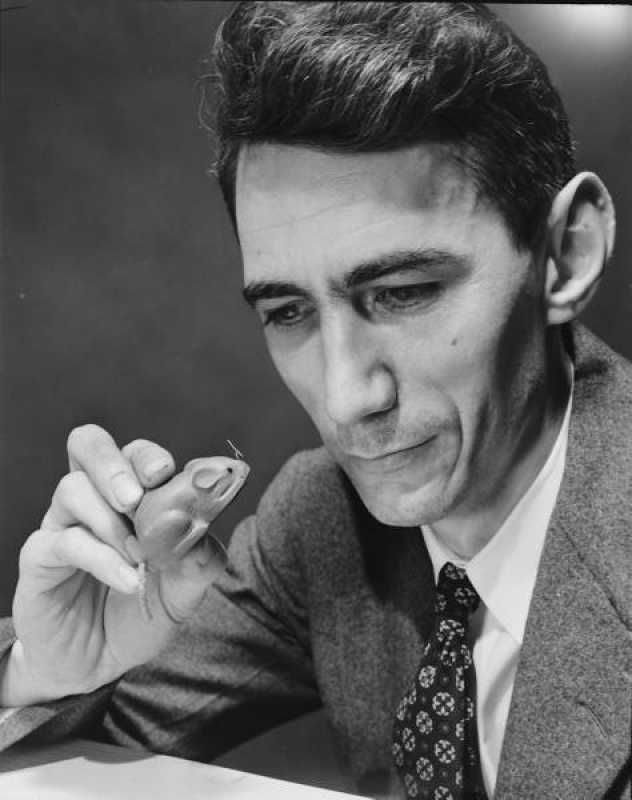
\includegraphics[scale=0.3]{images/Claude_Shannon_1776.jpg}\\
			\imagesource{DobriZheglov, CC BY-SA 4.0, via Wikimedia Commons.}
		\end{tabular}
	\end{center}
	\vspace*{-0.7em}
	\caption{Picture of Claude E. Shannon staring at a mouse.}
	\label{fig:shannon}
\end{figure}

\section{Huffman coding}
\begin{comment}
Òptim, prefix, FLAC, etc. Es compararà amb l'algoritme WAVE de FAPEC a través del rendiment de FLAC per àudio lossless.
\end{comment}

\section{Golomb coding}
\begin{comment}
Els codis de Rice (subconjunt dels codis de Golomb) van donar origen a FAPEC, així que és important comentar-los.
També són codis de prefix com el Huffman però poden no ser òptims.
\end{comment}

\section{Arithmetic coding}
\begin{comment}
Aquesta secció la faré servir per donar pas a l'Asymmetric numeral systems. Bàsicament els codis aritmètics són molt bons però són molt lents. Això ho compensa els ANS.
\end{comment}

\section{Asymmetric Numeral Systems}
\begin{comment}
Em centraré especialment en el Zstandard (Facebook). Tenen nivells de compressió similars als aritmètics però van MOLT ràpid (una mica més que FAPEC i tot).
\end{comment}
\chapter{The FAPEC Data Compressor}
En aquest capítol faré una explicació teòrica del FAPEC. Tota la informació que donaré ja està publicada en papers \parencite{PaperFAPEC} o a la patent americana de FAPEC \parencite{PatentFAPEC}. D'aquesta manera no hi ha problemes de confidencialitat i el TFG podrà ser públic.
\chapter{Development of new stages}
New \acrshort{fapec} stages must be well documented, efficient and easy to maintain. In order to achieve this, all stages are subject to some general requirements and must be evaluated. In this chapter we will first list the general requirements for new stages. Then, we will present four metrics to evaluate each stage.

\section{Requirements for \acrshort{fapec} stages} \label{sec:fapec_reqs}
In this section we will list the general requirements that all \acrshort{fapec} stages developed by DAPCOM must fulfill. Besides these, other specific requirements for each stage may be defined.

\subsubsection{Requirements} \label{sec:requirements}
\begin{enumerate}
	\item The stage must be implemented in C. \label{req:c}
	\item The software shall be provided as a library and as a stand-alone binary. \label{req:lib_bin}
	\item The stage must be able to work with data chunks. \label{req:chunks}
	\item The stage must support lossless and lossy compression.
	\item Data must not be lost even if the input is corrupted (i.e. delta fallback).
	\item Compression ratio shall be better than Gzip's.
	\item Compression speed shall be better than Gzip's.
	\item The software shall be tested with a representative dataset.
	\item The design and implementation must be documented.
\end{enumerate}

\subsubsection{Specifications}
The following specifications shall be fulfilled with an Intel Core i7-10710U \acrshort{cpu}.

\begin{enumerate}
	\item The occupied memory with one thread shall not exceed 64 MB.
	\item \acrshort{fapec} data chunks shall have a size between 128 kB and 4 MB.
	\item Decompression time can't be higher than a 110\% of the compression time.
	\item At least a 10\% of the source code lines must be comments.
	\item McCabe complexity \parencite{mccabe} shall be below 50.
\end{enumerate}

\section{Evaluation of stages}
The aim of this section is to present the metrics used in the following chapters to evaluate the developed preprocessing stages. The proposed indexes may be classified in two groups: information metrics and performance metrics.

\subsection{Information metrics}
This subset of metrics is purely focused on evaluating how better data are after the decorrelation stage. Our first approach is to plot a \textbf{histogram} of the original samples together with a histogram of the prediction errors (i.e. the values that will be sent to the \acrshort{fapec} entropy coder). For a better visualization, the bin width is calculated from the number of samples and it is the same for both histograms. Besides, the prediction errors histogram is also doted with three vertical lines at percentiles 5, 50 and 95 in order to clearly show the range where 90\% of data is contained.

Making use of the histograms, the \textbf{cumulative histograms} of the original samples and the prediction errors are calculated and plotted together. Although this graphics are just the integral of the histograms described above, they provide a clear way to see samples concentration in intervals.

\begin{figure}[h!]
	\centering
	\begin{subfigure}{0.5\textwidth}
		\centering
		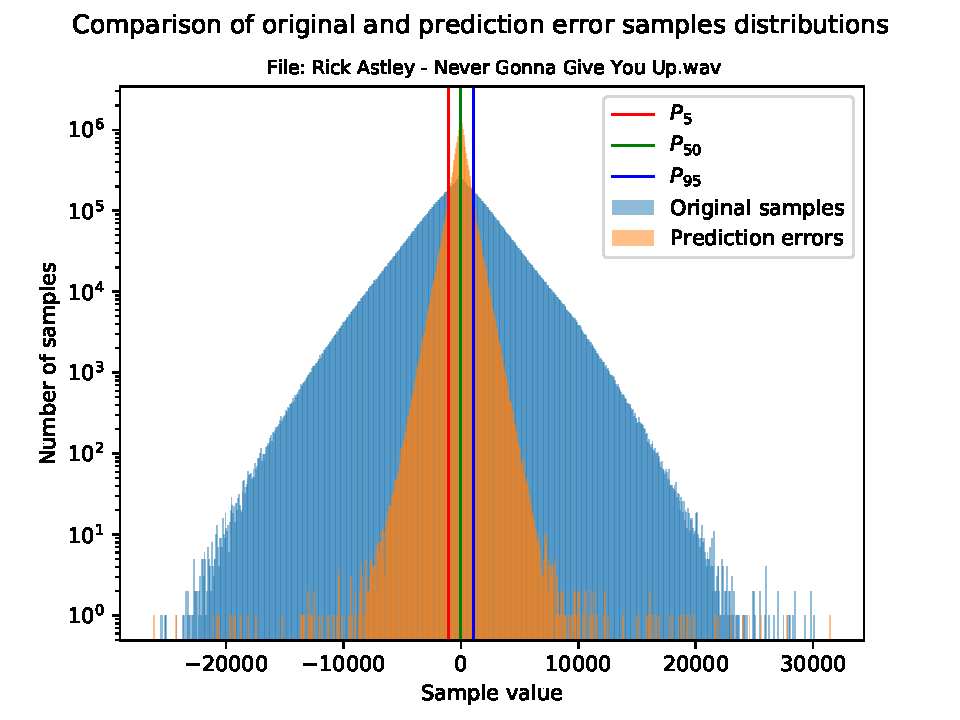
\includegraphics[width=\linewidth]{images/Rick Astley - Never Gonna Give You Up.wav_hist.pdf}
		\caption{Histogram of an audio file.}
		\label{fig:hist_example}
	\end{subfigure}%
	\begin{subfigure}{0.5\textwidth}
		\centering
		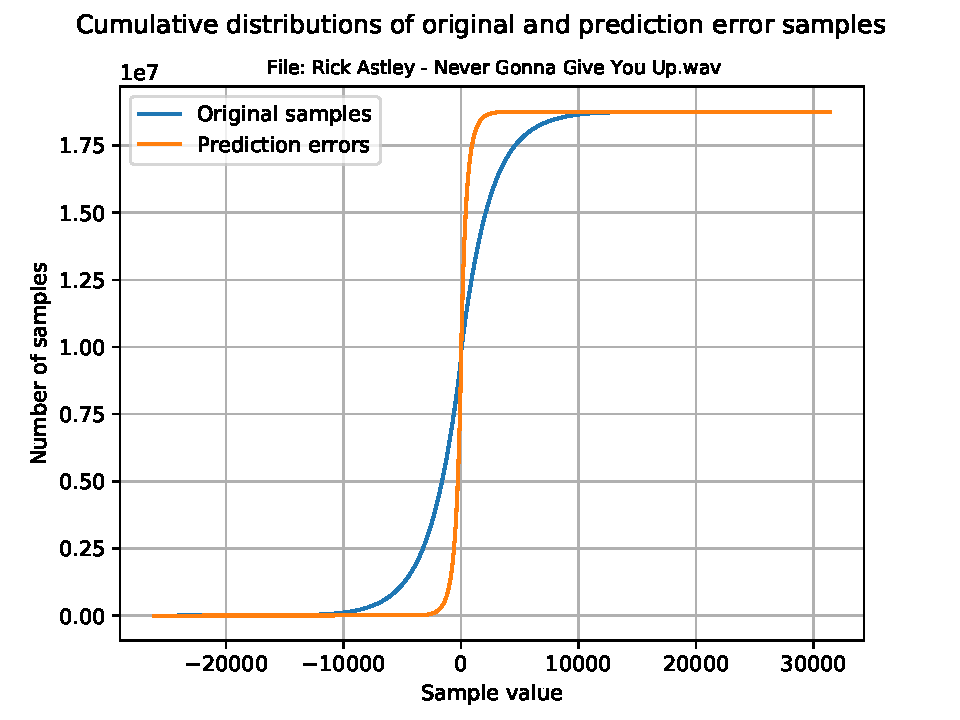
\includegraphics[width=\linewidth]{images/Rick Astley - Never Gonna Give You Up.wav_hist_cum.pdf}
		\caption{Cumulative histogram of an audio file.}
		\label{fig:sub2}
	\end{subfigure}
	\caption{Histogram and cumulative histogram of a file compressed with Wave.}
	\label{fig:test}
\end{figure}

At the beginning of this thesis no more information metrics were planned, but we realized that these two are subject to data scaling. That is, with a simple division the metric can be adulterated. In order to deal with it, we also propose to use \textbf{negentropy} (see section \ref{sec:negentropy}) to measure how compressible the prediction errors are compared with the original samples. There are two main reasons behind choosing negentropy: the first is that it is invariant to linear maps, and the second is that it is a measure of non-Gaussianity. The first property solves the problem of data scaling, and the second one offers a way of knowing if the stage has improved data distribution (i.e. negentropy is higher).

Although negentropy is a highly suitable metric for our purposes, it has an important drawback: its calculation is computationally very complex. Moreover, estimating it from data requires estimating the probability density function of the samples to later plug it into the definition of differential entropy and finally subtracting it to the Gaussian entropy for the same variance. However, negentropy can be approximated with the following expression \parencite{HYVARINEN2000411}:
\begin{equation}
J(X) \propto \left[E[G(X)] - E[G(V)]\right]^2
\end{equation}
where $X$ is a random variable with $\mu = 0$ and $\sigma = 1$, $V \sim N(0,1)$ and $G(u)$ is a non-quadratic function. In our case, $X$ and $V$ will be data arrays and
\begin{equation}
G(u) = \ln \cosh u
\end{equation}

\subsection{Performance metrics}
We are interested in comparing the whole compression process: from opening the original file to writing the encoded one. In other words, we want to evaluate the performance of the decorrelation stage plus the entropy coder compared with other compressors.

In this thesis we propose a new metric based on Euclidean distance that takes into account the (normalized) process time and the (inverse) compression ratio. Mainly, given an input file, it consists in computing a dot in $\mathbb{R}^2$ where the first coordinate is the normalized process time and the second is the inverse of the compression ratio. Then, the Euclidean distance to the origin is computed for every algorithm and the one with the smallest distance is assumed to be the best. Formally, the coordinates for each compressor are given by
\begin{equation} \label{eq:dot_comp}
\mathbf{a} = \left(t, \frac{s_c}{s_o}\right)
\end{equation}

and the metric is
\begin{equation} \label{eq:metric_gamma}
\gamma = \left\Vert \mathbf{a} \right\Vert ^2 = t^2 + \left(\frac{s_c}{s_o}\right)^2
\end{equation}

where $t$ is the process time normalized by 1 second, $s_c$ the compressed file size in bytes and $s_o$ the original file size also in bytes.

In order to reliably calculate the compression time, each compressor is run as a child-process on a Python script. Then, time is taken before spawning the child-process and again after it exits. Subtracting the end time to the start time gives the process time which, divided by 1 second, is used in equations \ref{eq:dot_comp} and \ref{eq:metric_gamma}.

Finally, we want to point out that in the following chapters the metric $\gamma$ will be given together with a plot including the dot $\mathbf{a}$ for several input files and compressors.

\chapter{Wave Stage}
Aquesta etapa decorreladora està enfocada a dades amb 2 canals (àudio stereo, I/Q). El desenvolupament dins de l'empresa està especialment enfocat per un client, però per motius de confidencialitat inclouré una versió genèrica que es podrà comparar amb el FLAC. L'etapa fa servir LPC i posteriorment envia els errors de predicció al codificador entròpic.

L'algoritme és el "típic" per LPC i la resolució del sistema lineal resultant del predictor lineal \parencite{PSAVC} es fa amb Levinson-Durbin \parencite{LevinsonDurbin}, que aprofitant l'estructura Toeplitz redueix la complexitat de $O(n^3)$ a $O(n^2)$.

\section{Introduction}
Etapa per Spire però per motius de confidencialitat se n'han eliminat algunes parts i es presenta un algoritme genèric.

\section{Design}
Disseny del predictor i l'estructura de l'etapa. Justificació de per què s'utilitzen els LPC i no una altra cosa. La resolució de les equacions de Yule-Walker anirà aquí, però segurament en posaré la deducció en un annex.

\section{Implementation}
Implementació amb C de l'algoritme. El codi anirà als annexes (a poder ser confidencials).

\section{Results}
D'això ja tinc alguna cosa provada i amb la versió d'ara, amb la cançó Money de Pink Floyd quasi iguala el FLAC. Acceptant unes miques de pèrdues (jo no les distingeixo) el supera molt.
\chapter{KMALL Stage}
\begin{comment}
Aquesta etapa decorreladora està enfocada a dades provinents de sondes submarines de l'empresa KONGSBERG.

La informació més interessant dels fitxers .kmall (ordre dels 100 MB) és la de les columnes d'aigua (ocupa el 99\% de la mida total del fitxer). El format d'aquests fitxers està basat en datagrames, la documentació dels quals és pública a la web de KONGSBERG (com que és un dOxygen en un Zip cal veure com ho citem).

Com que FAPEC comprimeix per chunks s'ha de parar especial atenció a no partir un datagrama per la meitat.
\end{comment}

Recent advances in sonar technology and computing power have led to an improvement in ocean monitoring. For instance, Multibeam Echosounders (MBES) are now capable of collecting data from the water columns, besides some usual metrics as seafloor reflectivity. This new information allows geoscientists to identify sunken structures, schools of fish, gas seeps, etc.

\begin{figure}[h!]
	\begin{center}
		  \begin{tabular}{ @{} r @{} }
			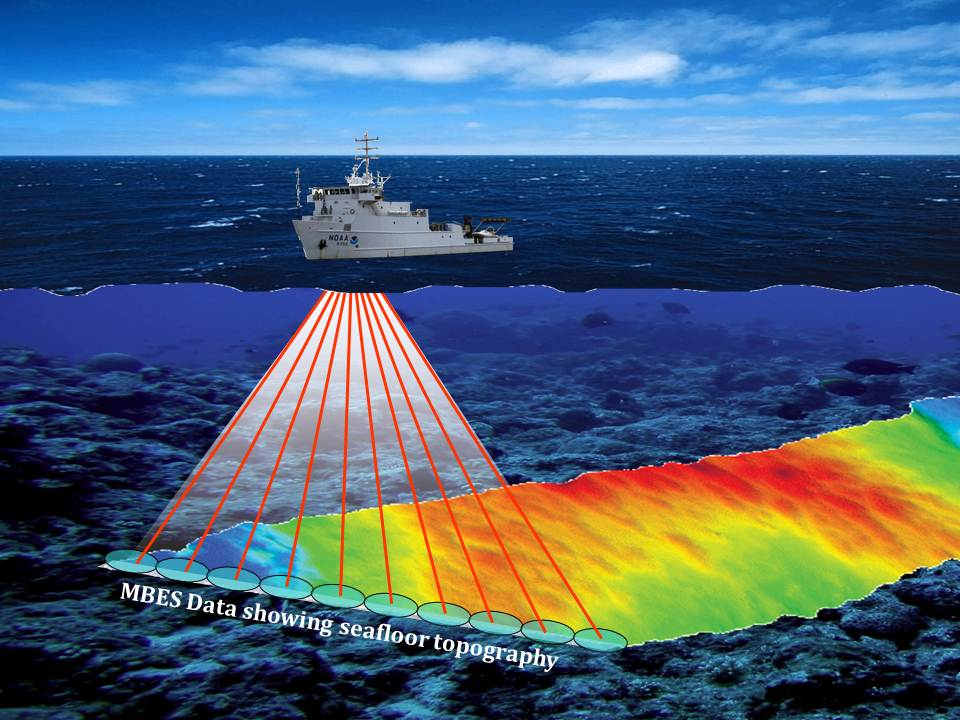
\includegraphics[scale=0.45]{images/mbes_ship.jpg}\\
			\imagesource{NOAA Photo Library, CC BY 2.0, via Wikimedia Commons.}
		\end{tabular}
	\end{center}
	\vspace*{-0.7em}
	\caption{Conception of multibeam sonar on NOAA Ship NANCY FOSTER.}
	\label{fig:mbes_ship}
\end{figure}

We clearly see that water column metrics have a big interest. However, their storage requirements are quite demanding (in the order of some GB/h), hence it is not possible to continuously record water column data. In this scenario, efficient compression algorithms will be essential.

At the present moment, one of the biggest echosounder manufacturers is Kongsberg Maritime. In this chapter we will focus on the development of a preprocessing stage specially designed for the KMALL files from Kongsberg. First, a general overview of the data structures will be given. Then, with this format in mind, a design criterion will be proposed and implemented. Finally, we will analyze its performance and compare it with other compression algorithms.

\section{The KMALL data format}
In this section we will describe the KMALL data structure and why there is a need to develop new compression algorithms for this format, but first some concepts related to echosounders must be defined:
\begin{itemize}
	\item \textbf{Ping:} A ping is defined as a number of pulses transmitted at approximately the same time.
	\item \textbf{Beam:} Each ping is formed by some pulses in different angles, which we call beams.
\end{itemize}

Notice that the number of beams per ping depends on each sonar model, and the numbers of samples per beam depends on the angle and on the depth.

\begin{comment}
This dependence can be seen in figure X.
Imatge de la paràbola dels beams, però la imatge hauria d'anar a la secció de disseny.
\end{comment}

The .kmall format is the successor of the Kongsberg .all format. Analyzing the latter is out of the scope of this project, yet we can state some of the improvements that KMALL brings. 

On the first hand, KMALL is a generic format with high resolution data and with a datagram structure designed to avoid breaking existing decoders when updating the data structure.

On the other hand, .all format used to have a datagram size constraint of 64 kB due to the maximum size of UDP packets, but .kmall files are designed to be stored "as is" and then fragmented if needed. Its main advantage is that pings are not splitted between datagrams.

A .kmall file is usually between 100 and 400 MB, and inside it there are several datagrams. This mixture of data types in the same file makes it difficult for standard compressors like \textit{Zip} to identify data statistics, therefore they don't perform as good as one could expect. In order to improve the compression ratio, we are interested in knowing how are those datagrams placed inside the file and how to identify them. From Kongsberg KMALL documentation, we know that all datagrams start with a generic header that contains datagram size in bytes and a 4-character identifier. In the current version (410224 Revision H), there exist the following datagram types:

\begin{table}[h!]
\begin{center}
\begin{tabular}{|l|l|l|}
	\hline
	\rowcolor[HTML]{9698ED} 
	\multicolumn{1}{|c|}{\cellcolor[HTML]{9698ED}Type code} & \multicolumn{1}{c|}{\cellcolor[HTML]{9698ED}Struct name} & \multicolumn{1}{c|}{\cellcolor[HTML]{9698ED}Description} \\ \hline
	\#IIP                                                   & EMdgmIIP\_def                                            & Installation and sensor parameters.                      \\ \hline
	\#IOP                                                   & EMdgmIOP\_def                                            & Runtime operator parameters.                             \\ \hline
	\#IBE                                                   & EMdgmIB\_def                                             & Built in test (BIST) error report.                       \\ \hline
	\#IBR                                                   & EMdgmIB\_def                                             & Built in test (BIST) reply.                              \\ \hline
	\#IBS                                                   & EMdgmIB\_def                                             & Built in test (BIST) short reply.                        \\ \hline
\end{tabular}
\end{center}
\caption{Installation and runtime datagrams of the KMALL format.}
\end{table}

\begin{table}[h!]
\begin{center}
\begin{tabular}{|l|l|l|}
	\hline
	\rowcolor[HTML]{9698ED} 
	\multicolumn{1}{|c|}{\cellcolor[HTML]{9698ED}Type code} & \multicolumn{1}{c|}{\cellcolor[HTML]{9698ED}Struct name} & \multicolumn{1}{c|}{\cellcolor[HTML]{9698ED}Description}                                      \\ \hline
	\#MRZ                                                   & EMdgmMRZ\_def                                            & \begin{tabular}[c]{@{}l@{}}Multibeam (M) raw range (R)\\ and depth (Z) datagram.\end{tabular} \\ \hline
	\#MWC                                                   & EMdgmMWC\_def                                            & \begin{tabular}[c]{@{}l@{}}Multibeam (M) water (W)\\ column (C) datagram.\end{tabular}        \\ \hline
\end{tabular}
\end{center}
\caption{Multibeam datagrams of the KMALL format.}
\end{table}

\begin{table}[h!]
\begin{center}
\begin{tabular}{|l|l|l|}
	\hline
	\rowcolor[HTML]{9698ED} 
	\multicolumn{1}{|c|}{\cellcolor[HTML]{9698ED}Type code} & \multicolumn{1}{c|}{\cellcolor[HTML]{9698ED}Struct name} & \multicolumn{1}{c|}{\cellcolor[HTML]{9698ED}Description}                                              \\ \hline
	\#SPO                                                   & EMdgmSPO\_def                                            & Sensor (S) data for position (PO).                                                                    \\ \hline
	\#SKM                                                   & EMdgmSKM\_def                                            & Sensor (S) KM binary sensor format.                                                                   \\ \hline
	\#SVP                                                   & EMdgmSVP\_def                                            & \begin{tabular}[c]{@{}l@{}}Sensor (S) data from sound velocity (V)\\ profile (P) or CTD.\end{tabular} \\ \hline
	\#SVT                                                   & EMdgmSVT\_def                                            & \begin{tabular}[c]{@{}l@{}}Sensor (S) data for sound velocity (V)\\ at transducer (T).\end{tabular}   \\ \hline
	\#SCL                                                   & EMdgmSCL\_def                                            & Sensor (S) data from clock (CL).                                                                      \\ \hline
	\#SDE                                                   & EMdgmSDE\_def                                            & Sensor (S) data from depth (DE) sensor.                                                               \\ \hline
	\#SHI                                                   & EMdgmSHI\_def                                            & Sensor (S) data for height (HI).                                                                      \\ \hline
\end{tabular}
\end{center}
\caption{External sensor output datagrams of the KMALL format.}
\end{table}

\begin{table}[h!]
\begin{center}
\begin{tabular}{|l|l|l|}
	\hline
	\rowcolor[HTML]{9698ED} 
	\multicolumn{1}{|c|}{\cellcolor[HTML]{9698ED}Type code} & \multicolumn{1}{c|}{\cellcolor[HTML]{9698ED}Struct name} & \multicolumn{1}{c|}{\cellcolor[HTML]{9698ED}Description} \\ \hline
	\#CPO                                                   & EMdgmCPO\_def                                            & Compatibility (C) data for position (PO).                \\ \hline
	\#CHE                                                   & EMdgmCHE\_def                                            & Compatibility (C) data for heave (HE).                   \\ \hline
\end{tabular}
\end{center}
\caption{Compatibility datagrams of the KMALL format.}
\end{table}

\begin{table}[h!]
\begin{center}
\begin{tabular}{|l|l|l|}
	\hline
	\rowcolor[HTML]{9698ED} 
	\multicolumn{1}{|c|}{\cellcolor[HTML]{9698ED}Type code} & \multicolumn{1}{c|}{\cellcolor[HTML]{9698ED}Struct name} & \multicolumn{1}{c|}{\cellcolor[HTML]{9698ED}Description} \\ \hline
	\#FCF                                                   & EMdgmFCF\_def                                            & Backscatter calibration (C) file (F) datagram.           \\ \hline
\end{tabular}
\end{center}
\caption{File datagrams of the KMALL format.}
\end{table}

As we will see in the next section, we are specially interested in MWC datagrams, which have the following structure:

\begin{figure}[ht]
	\begin{center}
		\scalebox{.565}{% Graphic for TeX using PGF
% Title: /home/aniol/Documents/Uni/Telecos/TFG/mwc_datagram.dia
% Creator: Dia v0.97+git
% CreationDate: Fri Feb 12 18:10:30 2021
% For: aniol
% \usepackage{tikz}
% The following commands are not supported in PSTricks at present
% We define them conditionally, so when they are implemented,
% this pgf file will use them.
\ifx\du\undefined
  \newlength{\du}
\fi
\setlength{\du}{15\unitlength}
\begin{tikzpicture}[even odd rule]
\pgftransformxscale{1.000000}
\pgftransformyscale{-1.000000}
\definecolor{dialinecolor}{rgb}{0.000000, 0.000000, 0.000000}
\pgfsetstrokecolor{dialinecolor}
\pgfsetstrokeopacity{1.000000}
\definecolor{diafillcolor}{rgb}{1.000000, 1.000000, 1.000000}
\pgfsetfillcolor{diafillcolor}
\pgfsetfillopacity{1.000000}
\pgfsetlinewidth{0.100000\du}
\pgfsetdash{}{0pt}
\pgfsetmiterjoin
\pgfsetbuttcap
{\pgfsetcornersarced{\pgfpoint{0.000000\du}{0.000000\du}}\definecolor{diafillcolor}{rgb}{1.000000, 1.000000, 1.000000}
\pgfsetfillcolor{diafillcolor}
\pgfsetfillopacity{1.000000}
\fill (2.100000\du,9.900000\du)--(2.100000\du,15.000000\du)--(52.000000\du,15.000000\du)--(52.000000\du,9.900000\du)--cycle;
}{\pgfsetcornersarced{\pgfpoint{0.000000\du}{0.000000\du}}\definecolor{dialinecolor}{rgb}{0.000000, 0.000000, 0.000000}
\pgfsetstrokecolor{dialinecolor}
\pgfsetstrokeopacity{1.000000}
\draw (2.100000\du,9.900000\du)--(2.100000\du,15.000000\du)--(52.000000\du,15.000000\du)--(52.000000\du,9.900000\du)--cycle;
}\pgfsetlinewidth{0.100000\du}
\pgfsetdash{}{0pt}
\pgfsetbuttcap
{
\definecolor{diafillcolor}{rgb}{0.000000, 0.000000, 0.000000}
\pgfsetfillcolor{diafillcolor}
\pgfsetfillopacity{1.000000}
% was here!!!
\definecolor{dialinecolor}{rgb}{0.000000, 0.000000, 0.000000}
\pgfsetstrokecolor{dialinecolor}
\pgfsetstrokeopacity{1.000000}
\draw (7.058330\du,9.850000\du)--(7.058330\du,15.031300\du);
}
% setfont left to latex
\definecolor{dialinecolor}{rgb}{0.000000, 0.000000, 0.000000}
\pgfsetstrokecolor{dialinecolor}
\pgfsetstrokeopacity{1.000000}
\definecolor{diafillcolor}{rgb}{0.000000, 0.000000, 0.000000}
\pgfsetfillcolor{diafillcolor}
\pgfsetfillopacity{1.000000}
\node[anchor=base,inner sep=0pt, outer sep=0pt,color=dialinecolor] at (4.516770\du,12.193700\du){Header};
% setfont left to latex
\definecolor{dialinecolor}{rgb}{0.000000, 0.000000, 0.000000}
\pgfsetstrokecolor{dialinecolor}
\pgfsetstrokeopacity{1.000000}
\definecolor{diafillcolor}{rgb}{0.000000, 0.000000, 0.000000}
\pgfsetfillcolor{diafillcolor}
\pgfsetfillopacity{1.000000}
\node[anchor=base,inner sep=0pt, outer sep=0pt,color=dialinecolor] at (4.516770\du,12.993700\du){20 \ensuremath{[}B\ensuremath{]}};
\pgfsetlinewidth{0.100000\du}
\pgfsetdash{}{0pt}
\pgfsetbuttcap
{
\definecolor{diafillcolor}{rgb}{0.000000, 0.000000, 0.000000}
\pgfsetfillcolor{diafillcolor}
\pgfsetfillopacity{1.000000}
% was here!!!
\definecolor{dialinecolor}{rgb}{0.000000, 0.000000, 0.000000}
\pgfsetstrokecolor{dialinecolor}
\pgfsetstrokeopacity{1.000000}
\draw (10.606800\du,9.867080\du)--(10.606800\du,15.048300\du);
}
% setfont left to latex
\definecolor{dialinecolor}{rgb}{0.000000, 0.000000, 0.000000}
\pgfsetstrokecolor{dialinecolor}
\pgfsetstrokeopacity{1.000000}
\definecolor{diafillcolor}{rgb}{0.000000, 0.000000, 0.000000}
\pgfsetfillcolor{diafillcolor}
\pgfsetfillopacity{1.000000}
\node[anchor=base,inner sep=0pt, outer sep=0pt,color=dialinecolor] at (8.850100\du,12.193800\du){Partition};
% setfont left to latex
\definecolor{dialinecolor}{rgb}{0.000000, 0.000000, 0.000000}
\pgfsetstrokecolor{dialinecolor}
\pgfsetstrokeopacity{1.000000}
\definecolor{diafillcolor}{rgb}{0.000000, 0.000000, 0.000000}
\pgfsetfillcolor{diafillcolor}
\pgfsetfillopacity{1.000000}
\node[anchor=base,inner sep=0pt, outer sep=0pt,color=dialinecolor] at (8.850100\du,12.993800\du){4 \ensuremath{[}B\ensuremath{]}};
\pgfsetlinewidth{0.100000\du}
\pgfsetdash{}{0pt}
\pgfsetbuttcap
{
\definecolor{diafillcolor}{rgb}{0.000000, 0.000000, 0.000000}
\pgfsetfillcolor{diafillcolor}
\pgfsetfillopacity{1.000000}
% was here!!!
\definecolor{dialinecolor}{rgb}{0.000000, 0.000000, 0.000000}
\pgfsetstrokecolor{dialinecolor}
\pgfsetstrokeopacity{1.000000}
\draw (15.140100\du,9.867080\du)--(15.140100\du,15.048300\du);
}
% setfont left to latex
\definecolor{dialinecolor}{rgb}{0.000000, 0.000000, 0.000000}
\pgfsetstrokecolor{dialinecolor}
\pgfsetstrokeopacity{1.000000}
\definecolor{diafillcolor}{rgb}{0.000000, 0.000000, 0.000000}
\pgfsetfillcolor{diafillcolor}
\pgfsetfillopacity{1.000000}
\node[anchor=base,inner sep=0pt, outer sep=0pt,color=dialinecolor] at (12.883400\du,12.193800\du){CmnPart};
% setfont left to latex
\definecolor{dialinecolor}{rgb}{0.000000, 0.000000, 0.000000}
\pgfsetstrokecolor{dialinecolor}
\pgfsetstrokeopacity{1.000000}
\definecolor{diafillcolor}{rgb}{0.000000, 0.000000, 0.000000}
\pgfsetfillcolor{diafillcolor}
\pgfsetfillopacity{1.000000}
\node[anchor=base,inner sep=0pt, outer sep=0pt,color=dialinecolor] at (12.883400\du,12.993800\du){12 \ensuremath{[}B\ensuremath{]}};
\pgfsetlinewidth{0.100000\du}
\pgfsetdash{}{0pt}
\pgfsetbuttcap
{
\definecolor{diafillcolor}{rgb}{0.000000, 0.000000, 0.000000}
\pgfsetfillcolor{diafillcolor}
\pgfsetfillopacity{1.000000}
% was here!!!
\definecolor{dialinecolor}{rgb}{0.000000, 0.000000, 0.000000}
\pgfsetstrokecolor{dialinecolor}
\pgfsetstrokeopacity{1.000000}
\draw (19.780100\du,9.857080\du)--(19.780100\du,15.038300\du);
}
% setfont left to latex
\definecolor{dialinecolor}{rgb}{0.000000, 0.000000, 0.000000}
\pgfsetstrokecolor{dialinecolor}
\pgfsetstrokeopacity{1.000000}
\definecolor{diafillcolor}{rgb}{0.000000, 0.000000, 0.000000}
\pgfsetfillcolor{diafillcolor}
\pgfsetfillopacity{1.000000}
\node[anchor=base,inner sep=0pt, outer sep=0pt,color=dialinecolor] at (17.483400\du,12.193700\du){TxInfo};
% setfont left to latex
\definecolor{dialinecolor}{rgb}{0.000000, 0.000000, 0.000000}
\pgfsetstrokecolor{dialinecolor}
\pgfsetstrokeopacity{1.000000}
\definecolor{diafillcolor}{rgb}{0.000000, 0.000000, 0.000000}
\pgfsetfillcolor{diafillcolor}
\pgfsetfillopacity{1.000000}
\node[anchor=base,inner sep=0pt, outer sep=0pt,color=dialinecolor] at (17.483400\du,12.993700\du){12 \ensuremath{[}B\ensuremath{]}};
\pgfsetlinewidth{0.100000\du}
\pgfsetdash{}{0pt}
\pgfsetbuttcap
{
\definecolor{diafillcolor}{rgb}{0.000000, 0.000000, 0.000000}
\pgfsetfillcolor{diafillcolor}
\pgfsetfillopacity{1.000000}
% was here!!!
\definecolor{dialinecolor}{rgb}{0.000000, 0.000000, 0.000000}
\pgfsetstrokecolor{dialinecolor}
\pgfsetstrokeopacity{1.000000}
\draw (27.206700\du,9.865000\du)--(27.206700\du,15.046200\du);
}
% setfont left to latex
\definecolor{dialinecolor}{rgb}{0.000000, 0.000000, 0.000000}
\pgfsetstrokecolor{dialinecolor}
\pgfsetstrokeopacity{1.000000}
\definecolor{diafillcolor}{rgb}{0.000000, 0.000000, 0.000000}
\pgfsetfillcolor{diafillcolor}
\pgfsetfillopacity{1.000000}
\node[anchor=base,inner sep=0pt, outer sep=0pt,color=dialinecolor] at (23.516700\du,12.158400\du){SectorData};
% setfont left to latex
\definecolor{dialinecolor}{rgb}{0.000000, 0.000000, 0.000000}
\pgfsetstrokecolor{dialinecolor}
\pgfsetstrokeopacity{1.000000}
\definecolor{diafillcolor}{rgb}{0.000000, 0.000000, 0.000000}
\pgfsetfillcolor{diafillcolor}
\pgfsetfillopacity{1.000000}
\node[anchor=base,inner sep=0pt, outer sep=0pt,color=dialinecolor] at (23.516700\du,12.958400\du){9 x 16 \ensuremath{[}B\ensuremath{]}};
\pgfsetlinewidth{0.100000\du}
\pgfsetdash{}{0pt}
\pgfsetbuttcap
{
\definecolor{diafillcolor}{rgb}{0.000000, 0.000000, 0.000000}
\pgfsetfillcolor{diafillcolor}
\pgfsetfillopacity{1.000000}
% was here!!!
\definecolor{dialinecolor}{rgb}{0.000000, 0.000000, 0.000000}
\pgfsetstrokecolor{dialinecolor}
\pgfsetstrokeopacity{1.000000}
\draw (32.580000\du,9.855000\du)--(32.580000\du,15.036200\du);
}
% setfont left to latex
\definecolor{dialinecolor}{rgb}{0.000000, 0.000000, 0.000000}
\pgfsetstrokecolor{dialinecolor}
\pgfsetstrokeopacity{1.000000}
\definecolor{diafillcolor}{rgb}{0.000000, 0.000000, 0.000000}
\pgfsetfillcolor{diafillcolor}
\pgfsetfillopacity{1.000000}
\node[anchor=base,inner sep=0pt, outer sep=0pt,color=dialinecolor] at (29.950000\du,12.158300\du){RxInfo};
% setfont left to latex
\definecolor{dialinecolor}{rgb}{0.000000, 0.000000, 0.000000}
\pgfsetstrokecolor{dialinecolor}
\pgfsetstrokeopacity{1.000000}
\definecolor{diafillcolor}{rgb}{0.000000, 0.000000, 0.000000}
\pgfsetfillcolor{diafillcolor}
\pgfsetfillopacity{1.000000}
\node[anchor=base,inner sep=0pt, outer sep=0pt,color=dialinecolor] at (29.950000\du,12.958300\du){16 \ensuremath{[}B\ensuremath{]}};
% setfont left to latex
\definecolor{dialinecolor}{rgb}{0.000000, 0.000000, 0.000000}
\pgfsetstrokecolor{dialinecolor}
\pgfsetstrokeopacity{1.000000}
\definecolor{diafillcolor}{rgb}{0.000000, 0.000000, 0.000000}
\pgfsetfillcolor{diafillcolor}
\pgfsetfillopacity{1.000000}
\node[anchor=base,inner sep=0pt, outer sep=0pt,color=dialinecolor] at (42.150000\du,12.125000\du){BeamData};
% setfont left to latex
\definecolor{dialinecolor}{rgb}{0.000000, 0.000000, 0.000000}
\pgfsetstrokecolor{dialinecolor}
\pgfsetstrokeopacity{1.000000}
\definecolor{diafillcolor}{rgb}{0.000000, 0.000000, 0.000000}
\pgfsetfillcolor{diafillcolor}
\pgfsetfillopacity{1.000000}
\node[anchor=base,inner sep=0pt, outer sep=0pt,color=dialinecolor] at (42.150000\du,12.925000\du){$N_B \cdot (16 + N_S \cdot (1 + phaseFlag))$ \ensuremath{[}B\ensuremath{]}};
\end{tikzpicture}
}
	\end{center}
	\caption{MWC datagram as described by Kongsberg (410224 Revision H).}
	\label{fig:mwc_datagram}
\end{figure}

Where:
\begin{description}
	\item $N_B \equiv$ Number of beams in ping. It is stored as a 16-bit integer in \textit{RxInfo}.
	\item $N_S \equiv$ Number of samples in beam. It is stored as a 16-bit integer in \textit{BeamData}.
	\item $phaseFlag \equiv$ Flag that indicates if there is phase information after amplitude samples. It may be 0 (no phase information), 1 (low resolution) or 2 (high resolution). It is stored as an 8-bit integer in \textit{RxInfo}.
\end{description}

\begin{comment}
Caldria comentar més els camps del datagrama o així està bé?
\end{comment}

It is important to notice that even though .kmall files can contain all the above datagrams, usually water column data is logged in a separate file with extension .kmwcd. In other words, MWC datagrams will be placed in .kmwcd files instead of .kmall files, but the decoding process is the same for both extensions.

\section{Design}
\begin{comment}
Potser hauria de fer subseccions? "Datagrams to compress", "Criteria", etc.
\end{comment}

In the previous section we introduced the KMALL data format. Namely, we saw that it is a mixture of different data types, so we have to decide which ones should be compressed and which algorithm will be applied.

In order to decide what to compress, we have first analyzed some .kmall and .kmwcd to determine the percentage of occupancy by datagram type. For the former files, we found that MRZ datagrams are a 92\% of the total size; and for the later, MWC datagrams are a 99\%. It is clear that these two data types are our objective; however, in this thesis we will ignore MRZ datagrams and we will just focus on MWC data. Actually, if we look at figure \ref{fig:mwc_datagram} we see that MWC headers are insignificant compared to its samples, therefore we will only compress payload information.

Once we have decided that we will restrict to water column data, a design criteria must be properly defined. This design has to take into account multiple aspects, namely: speed, implementation easiness and compression performance.

In previous chapters we explained that FAPEC compresses files by breaking them into chunks and processing each of them individually. This feature may be dangerous in our datagram scenario, so our first criterion will be to avoid FAPEC from splitting datagrams into different chunks. This way, the implementation will be much easier at the cost of reducing the process performance.

\begin{comment}
Estic anant massa per feina i sent poc curós, així que afegeixo la resta de criteris com a comentari i ja ho redactaré un altre dia.

Degut a l'estructura "parabòlica" de les mostres (pendent generar figura), cal vigilar en com les processem. La proposta és: per la secció quadrada restem respecte beam anterior (molt semblants). Per la secció parabòlica comprovem la diferència de mostres amb l'anterior i amb el simètric. Les opcions d'això són:

difAnt = 0, difSim = 0 => Ant\\
difAnt != 0, difSim != 0 => Ant\\
difAnt != 0, difSim = 0 => Sim

El motiu d'això és que està més correlat amb l'anterior i també cal més padding (el nombre de mostres entre beams decreix quadràticament), cosa bona per FAPEC (millor afegir 10 zeros que 2).
\end{comment}

\section{Implementation}
\begin{comment}
Implementació amb C de l'algoritme. El codi anirà als annexes (a poder ser confidencials).
\end{comment}

\section{Results}
\begin{comment}
No ens precipitem.
\end{comment}
\chapter{Conclusions and Future Work}
Això no toca.

\printbibliography[heading=bibintoc]

\begin{appendices}
\chapter{Proof of Equation \ref{eq:differential_entropy_q}}\label{entropy_proof}

In some papers such as \parencite{Vasicek} the authors use Equation \ref{eq:differential_entropy_q} instead of Equation \ref{eq:differential_entropy}, but no formal proof is included. In this appendix we provide a clear proof which shows that equations \ref{eq:differential_entropy} and \ref{eq:differential_entropy_q} are equivalent.

Let $X$ be a continuous random variable with cumulative distribution function $F(x)$. Then, its quantile function is defined as:
\begin{equation}
Q(p) = F^{-1}(p) = \inf\{x \in \mathbb{R} : p \leq F(x)\}
\end{equation}
for a probability $0 \leq p \leq 1$.

From the previous definition we obtain:
\begin{align} 
F(x) = F(Q(p)) = p \label{eq:quantile_cdf} \\ 
Q(p) = Q(F(x)) = x \label{eq:cdf_quant}
\end{align}

Applying the chain rule to Equation \ref{eq:quantile_cdf}:
\begin{equation}\label{eq:cdf_identity}
\frac{dF(Q(p))}{dp} = \frac{dF(Q)}{dQ} \cdot \frac{dQ(p)}{dp} = f(Q(p)) \cdot Q'(p) = 1
\end{equation}

Now, take the differential entropy as defined in \ref{eq:differential_entropy} and, for simplicity, rewrite it as:
\begin{equation} \label{eq:u_entropy}
h(X) = - \int_{-\infty}^{+\infty} f(x) \ln f(x) dx = - \int_{-\infty}^{+\infty} u(x) dx
\end{equation}

Applying the change of variables from \ref{eq:cdf_quant} to \ref{eq:u_entropy} and remembering that $F(x)$ is monotonically increasing, we obtain the following integration limits:
\begin{align}
a = \lim_{x \to -\infty} F(x) = 0\\
b = \lim_{x \to +\infty} F(x) = 1
\end{align}

And the following integrand:
\begin{equation}
h(X) = - \int_{0}^{1} u(Q(p)) \cdot Q'(p) dp = - \int_{0}^{1} f(Q(p)) \cdot \ln(f(Q(p))) \cdot Q'(p) dp
\end{equation}
which, making use of Equation \ref{eq:cdf_identity}, can be simplified to Equation \ref{eq:differential_entropy_q}:
\begin{equation}
h(X) = -  \int_{0}^{1} \ln\left(f(Q(p))\right) dp = - \int_{0}^{1} \ln\left(\frac{1}{Q'(p)}\right) dp = \int_{0}^{1} \ln\left(Q'(p)\right) dp
\end{equation}
\hspace*{\fill}$\blacksquare$
\chapter{Linear Prediction}
Formulació del predictor lineal i equacions de Yule-Walker.
\chapter{Levinson-Durbin}
Algoritme de Levinson-Durbin utilitzat per resoldre sistemes lineals amb matrius Toeplitz.
\end{appendices}

\printacronyms

\end{document}          
